%!TEX root = ../../presentation.tex

\begin{frame}[plain]{Recall: Monitoring Program Flow Trace}
  \textwidthplain
  \centering
  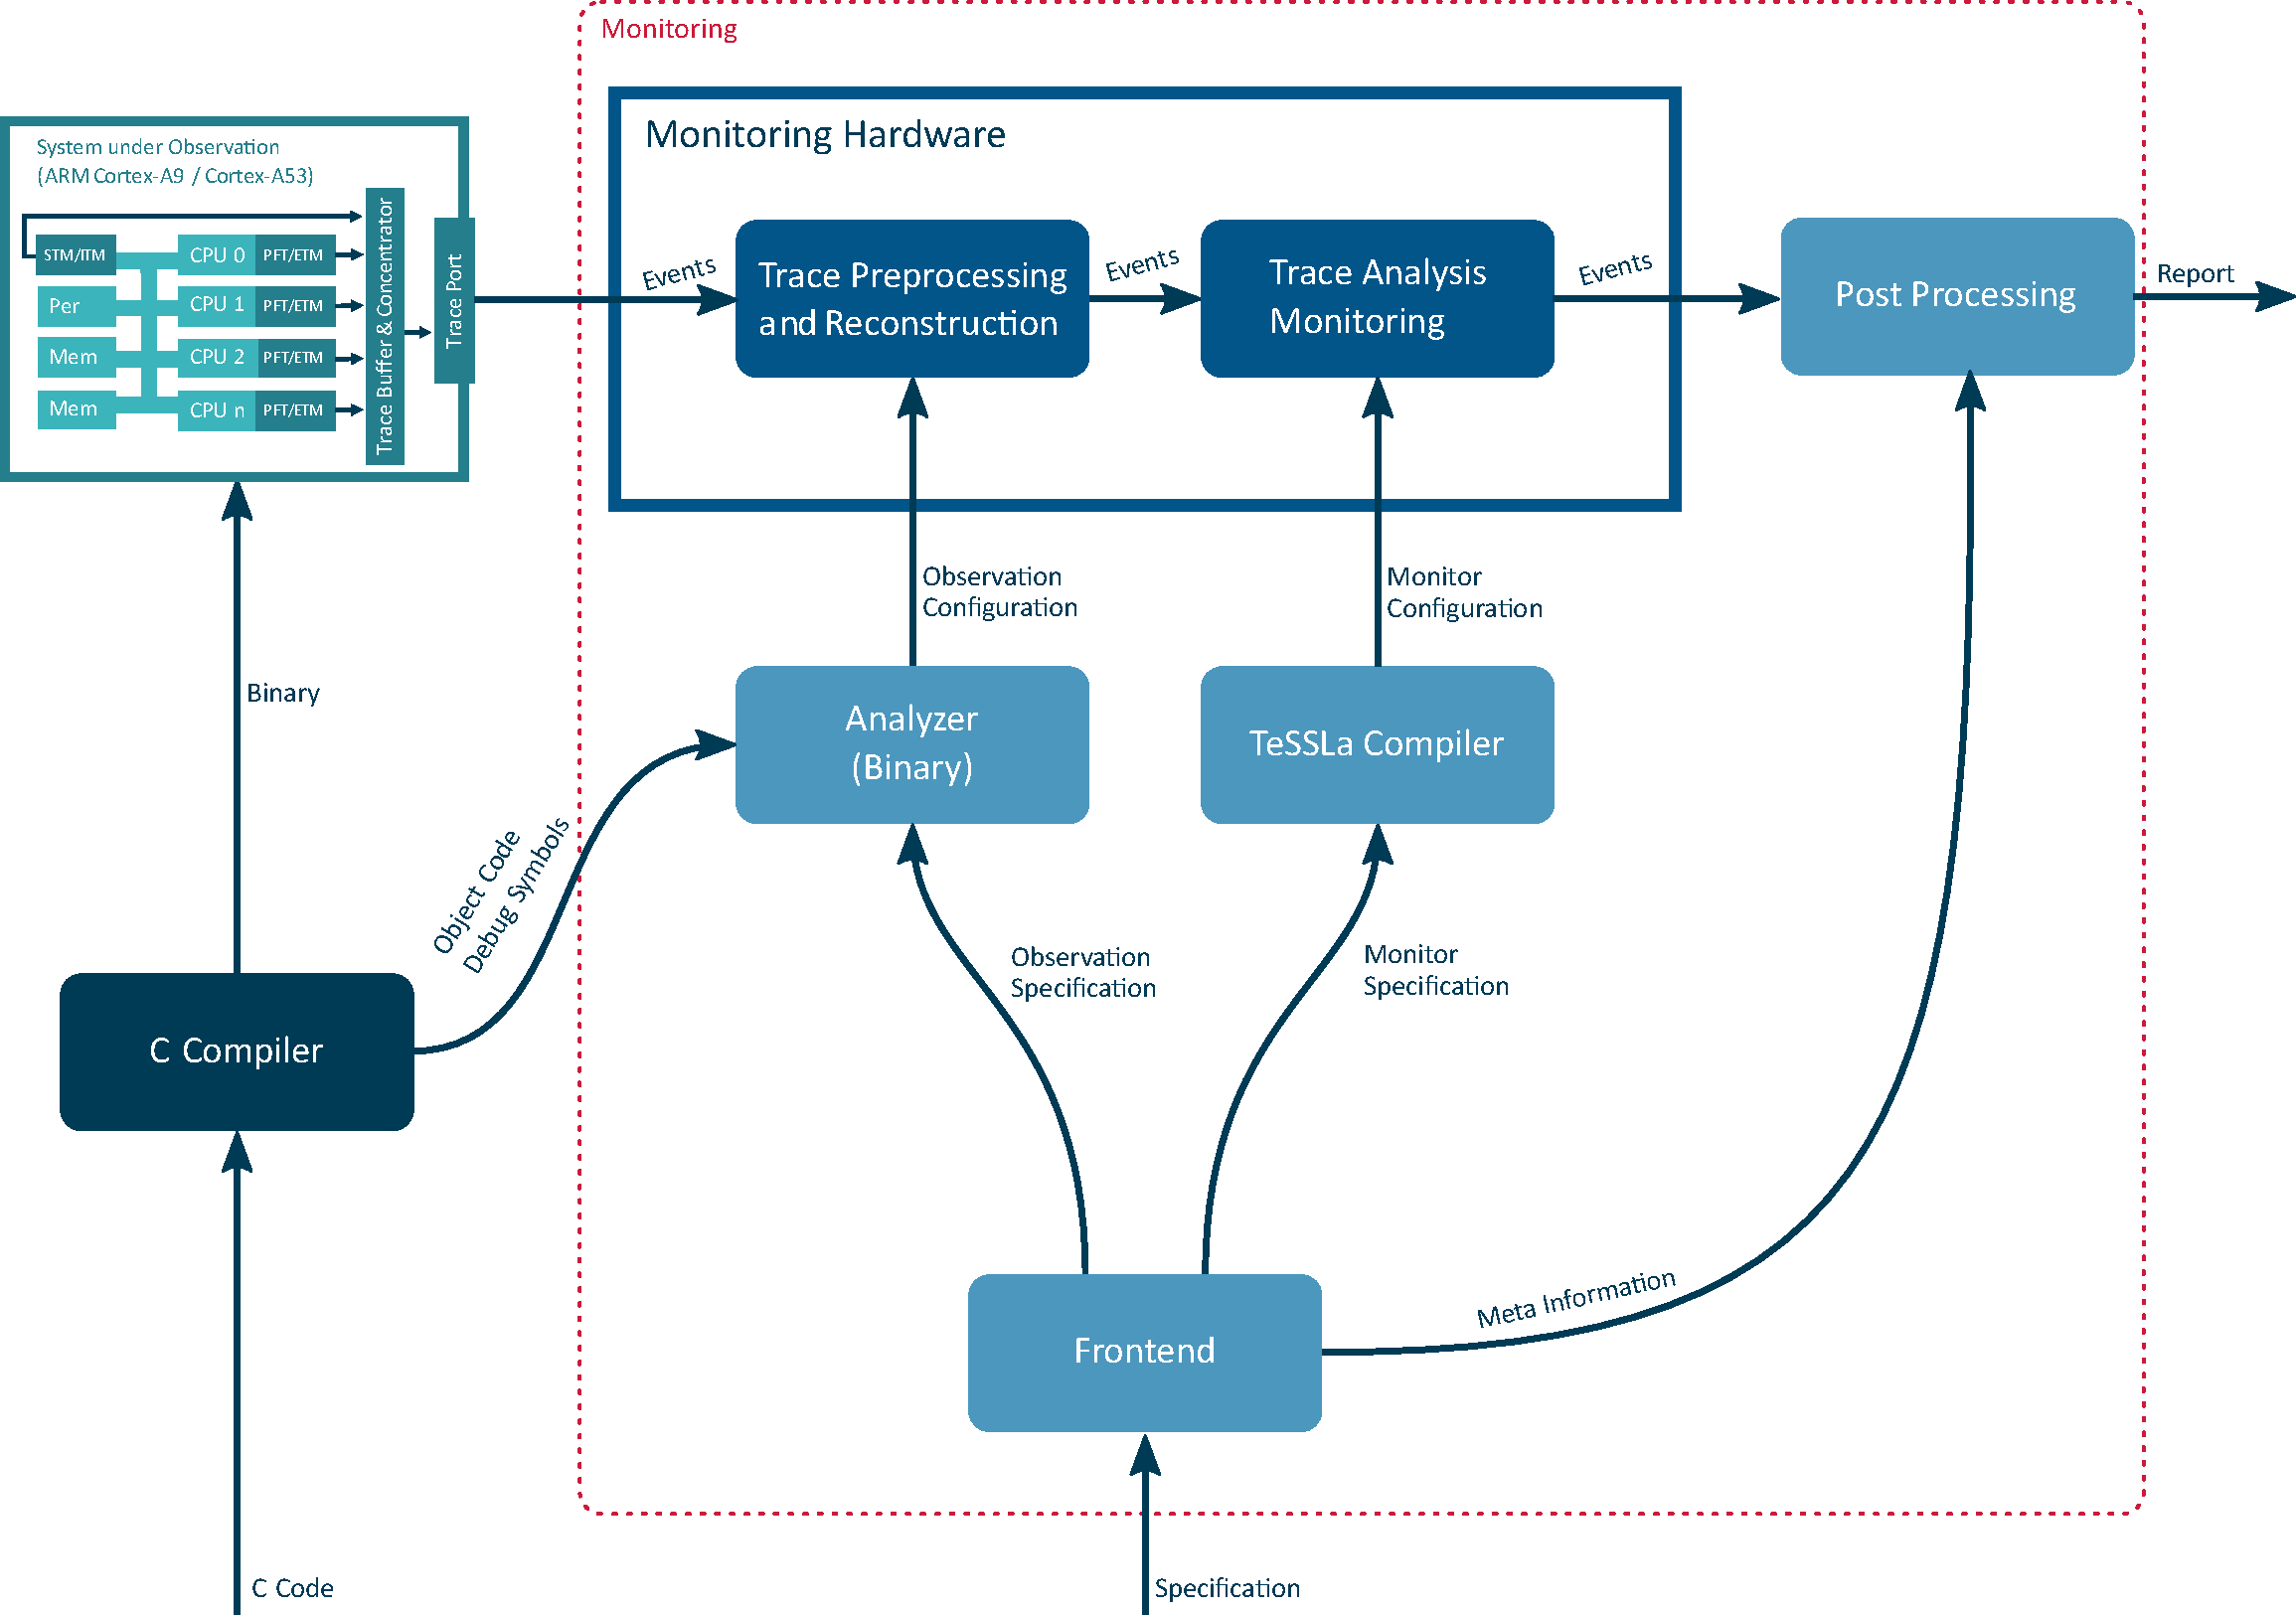
\includegraphics[width=.9\textwidth]{content/chapter_hardware_srv/overview-program-trace.pdf}
\end{frame}

\begin{frame}[plain]{Monitoring Data Values}
  \textwidthplain
  \centering
  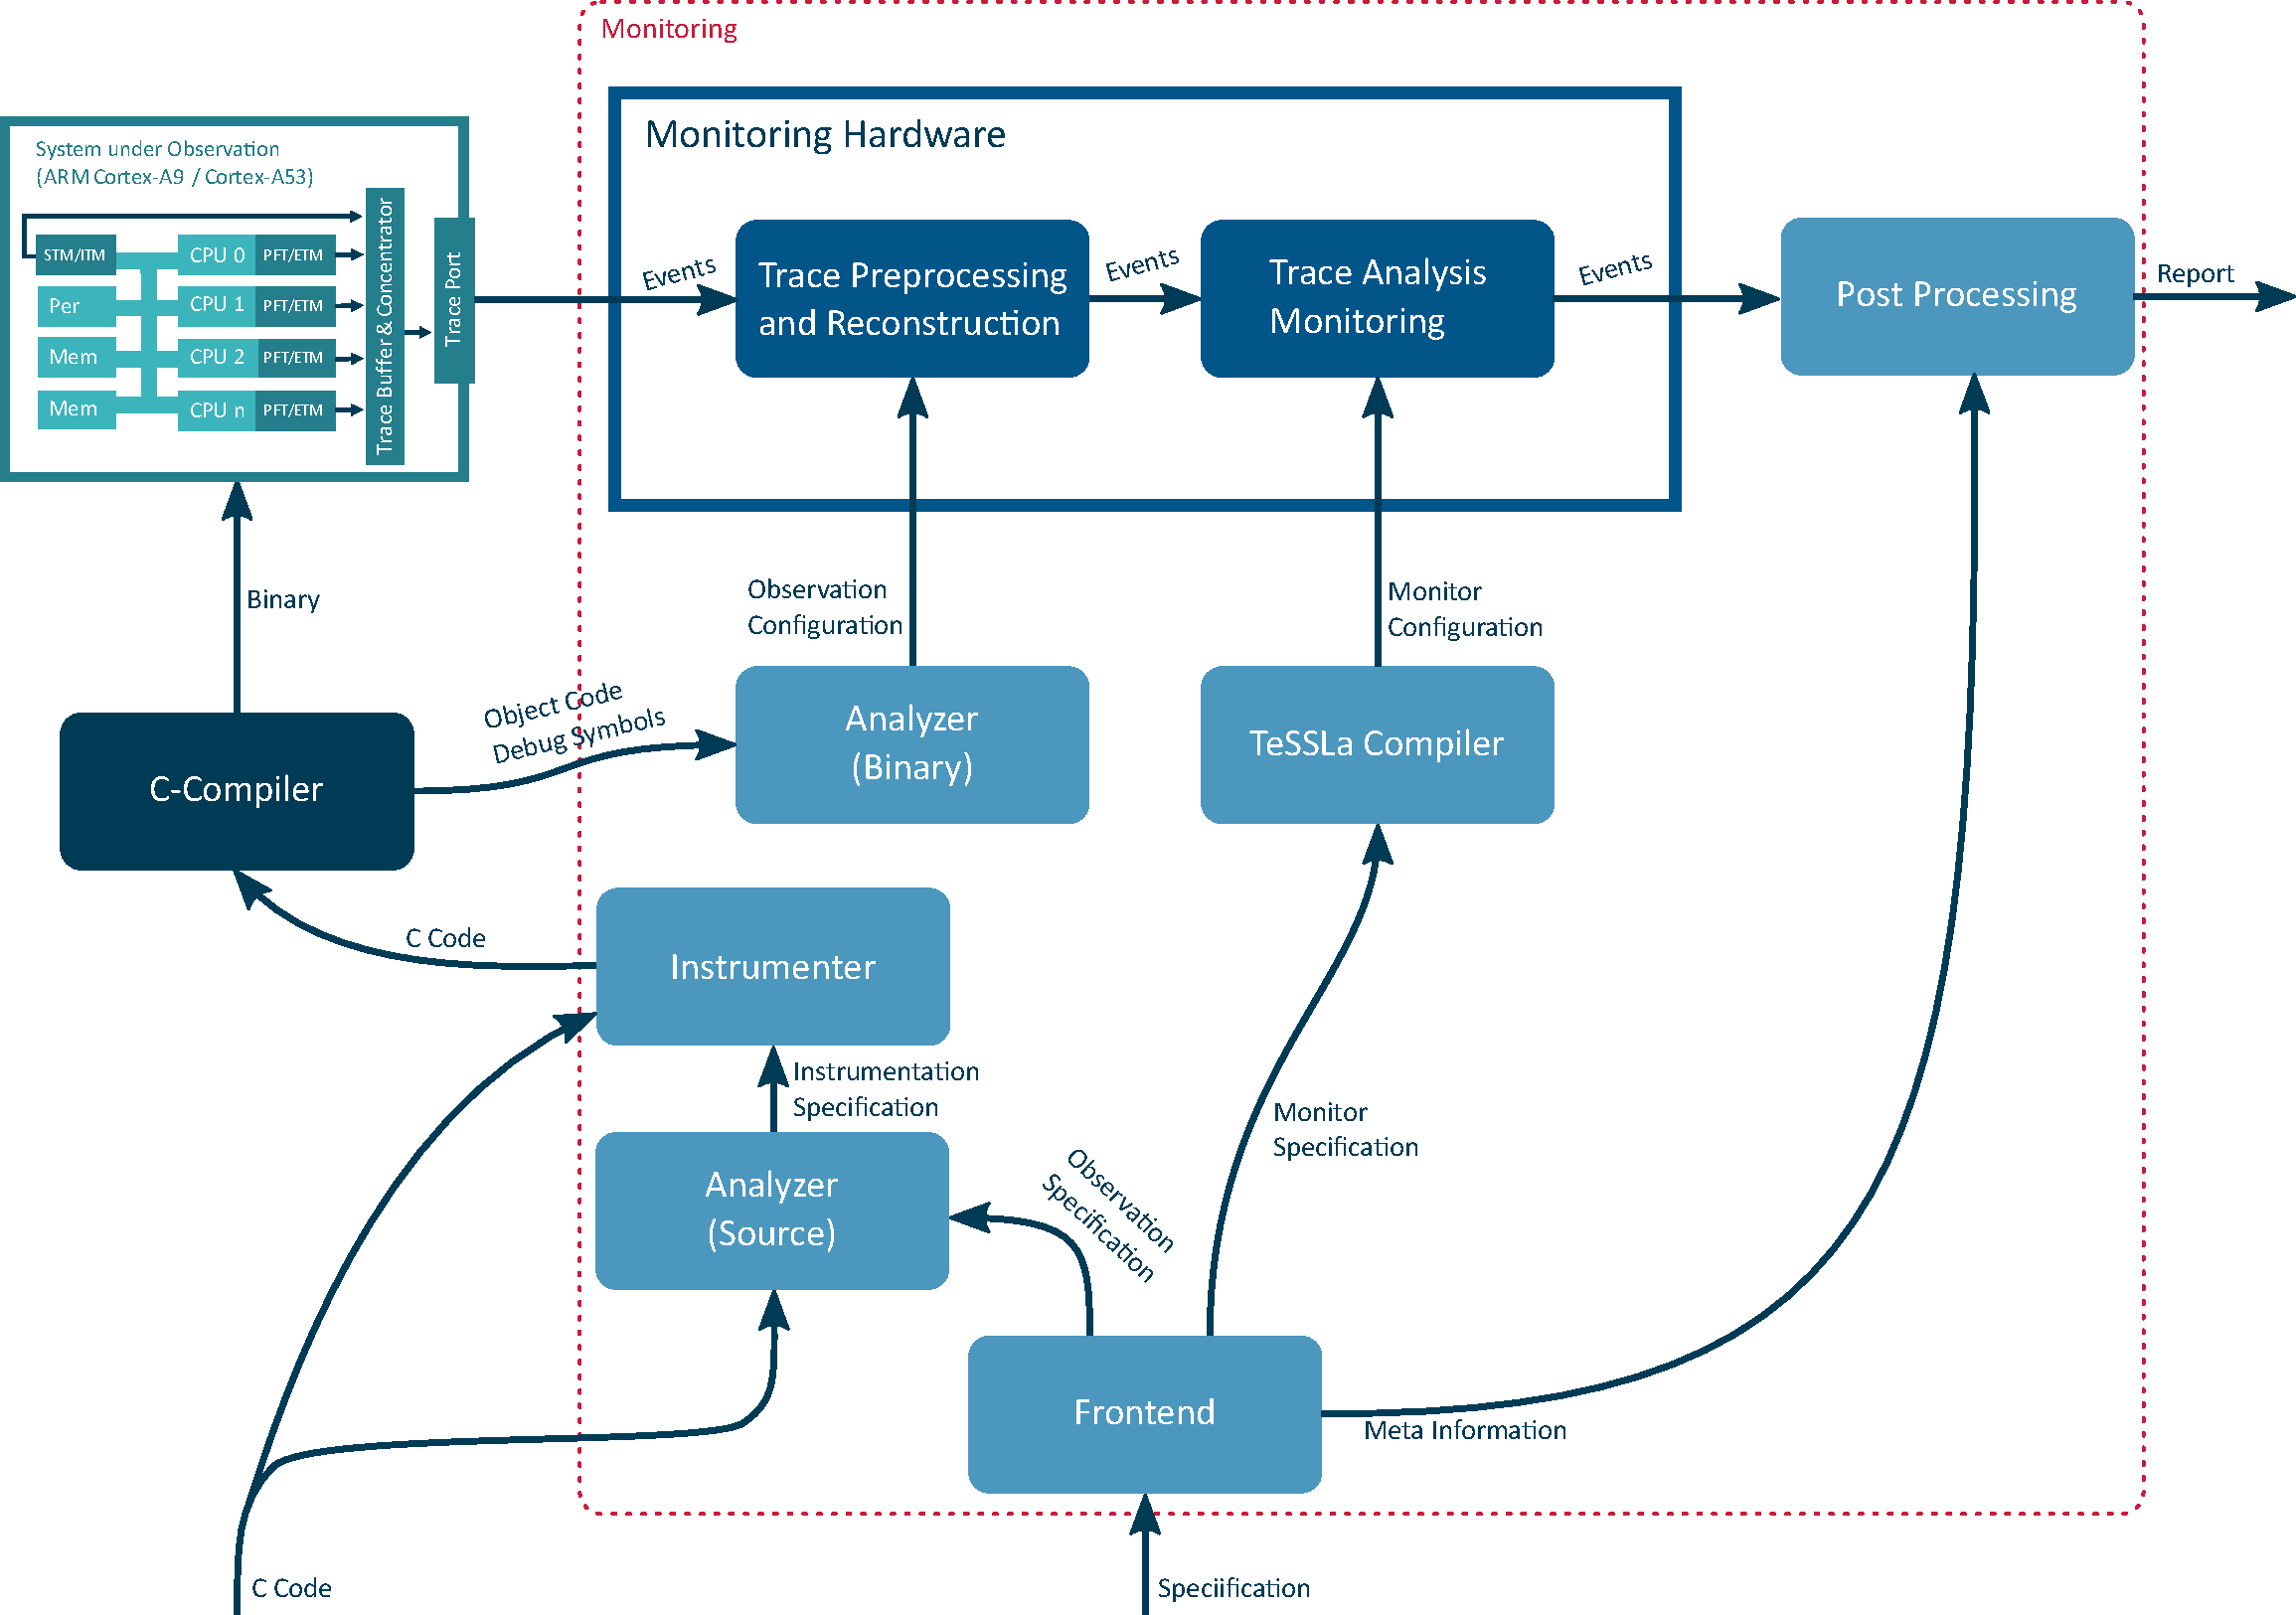
\includegraphics[width=.9\textwidth]{content/chapter_hardware_srv/overview-itm.pdf}
\end{frame}

\begin{frame}[fragile]{Monitoring the Speed Supervisor}
  \begin{block}{Property}
    23~s after the distant signal the allowed speed\\
    computed by the supervisor must be equal to 85~km/h.
  \end{block}

  \scriptsize

  \begin{lstlisting}[gobble=4,language=tessla]
    # Specify values we are interested in
    def signal := function_argument("getAllowedSpeed", 1)
    def allowed_speed := function_result("getAllowedSpeed")

    # Changes where signal becomes DISTANT_SIGNAL_CAUTION
    def caution := filter(changes(signal),
                        signal == DISTANT_SIGNAL_CAUTION)

    def valid :=
      # Either we are not yet 23s after the distant signal
      time(allowed_speed) - time(caution) <= 23s
      # or the allowed speed must be below 85~km/h
      || allowed_speed * 36 <= 85 * 1000
  \end{lstlisting}
\end{frame}

\begin{frame}[fragile]{Monitoring Data Value: How It Works}
  \scriptsize

  \begin{lstlisting}[gobble=4,language=tessla]
    # Specify values we are interested in
    def signal := function_argument("getAllowedSpeed", 1)
    def allowed_speed := function_result("getAllowedSpeed")
  \end{lstlisting}

  \xxx

  \begin{columns}
    \column{4.7cm}
    \inhead{Instrumented C Code}
    \vskip-3pt
      \begin{lstlisting}[gobble=6,language=C]
      double getAllowedSpeed(
          int signal, ...) {
        tessla_debug(1, (int64_t)
          signal);
        double result = ...
        tessla_debug(2, (int64_t)
          (result * 1000));
        return result;
      }
    \end{lstlisting}

    \column{4.7cm}
    \inhead{Updated Specification}
    \vskip-3pt
    \begin{lstlisting}[gobble=6,mathescape=true,language=tessla]
      in debug_slot: Events[Int]
      in debug_value: Events[Int]
      def signal :=
        filter(debug_value,
          debug_slot == 1)
      def allowed_speed :=
        filter(debug_value,
          debug_slot == 2)
          $~$
    \end{lstlisting}
  \end{columns}
\end{frame}
